\documentclass[aspectratio=43]{beamer}

\usetheme{simple}

\usepackage{lmodern}
\usepackage[scale=2]{ccicons}
\usepackage{multicol}

\usepackage[utf8]{inputenc}



% Info de la presentación
\def\edicion{XXXV}
\def\fecha{Abril 2023}

\title{Te has instalado Linux... ahora, ¿qué?} % título de la presentación
\author{Luis Daniel Casais} % autor de la presentación
\github{rajayonin} % GitHub

\institute{\edicion \ Jornadas Técnicas del GUL}
\date{\fecha}



% Cover
\titlegraphic{img/logo1.png}
\begin{document}

{
    \setbeamertemplate{footline}{}
    \begin{frame}
        \titlepage
    \end{frame}
}
\addtocounter{framenumber}{-1}


% Table of contents
\begin{frame}
    \frametitle{Tabla de contenidos}
    \begin{multicols}{2}
        \tableofcontents
    \end{multicols}
\end{frame}



% -----------------------------
% La presentación empieza aquí.
% -----------------------------


\section{Personalización}
% Desktop Enviroments / tiling window managers (i3) / tty
% Emuladores de terminal: kitty (bonito y simple, usa GPU), terminator (GUI friendly), alarcritty (moderno, usa GPU), iterm2 // tmux
% Shells: bash, zsh, fish
% Dotfiles: .bashrc, etc


\begin{frame}
    \frametitle{GUI (Graphical User Interface)}
    Por defecto, Linux cuenta con tres tipos principales de GUI: \textbf{Lockscreen} (pantalla de bloqueo), \textbf{Desktop Enviroment}, y \textbf{TTY/shell}.\newline

    Se puede acceder a cualquiera de ellos con las siguientes combinaciones de teclas:
    \begin{itemize}
        \item \texttt{CTRL + ALT + F1}: Lockscreen
        \item \texttt{CTRL + ALT + F2}: Desktop Environment
        \item \texttt{CTRL + ALT + F3}: TTY3
        \item \texttt{CTRL + ALT + F4}: TTY4\\
        ...\newline
    \end{itemize}
    
    Cualquiera de los tres tipos son personalizables e intercambiables, ya que \textbf{LINUX ES EL AMO Y SEÑOR DE LA PERSONALIZACIÓN}.
\end{frame}

\subsection{Desktop Enviroments}

\begin{frame}
    \frametitle{Desktop Enviroments}
    Es la principal forma de interacción con el ordenador.\\
    Todo lo que puedes ver y tocar (iconos, ventanas, \textit{toolbars}, \textit{wallpapers}, etc.) es parte del Desktop Enviroment.\newline

    Son todos intercambiables y, aunque la forma de hacerlo depende de la \textit{distro} específica, normalmente se pueden cambiar en la \textit{lockscreen}.\\
    Algunas \textit{distros} incluso te permiten elegir cual usar al instalar el SO.\newline

    Hay dos tipos principales, dependiendo de cómo manejan el uso de las ventanas: \textbf{Floating Window Managers} y \textbf{Tiling Window Managers}.
\end{frame}

\begin{frame}
    \frametitle{Floating Window Managers}
    La típica interfaz de un Sistema Operativo moderno, con ventanas "flotantes". Intuitivo y fácil de usar.\newline

    % images
    \begin{columns}[c]
        \begin{column}{0.5\textwidth}
            \begin{figure}
                \centering
                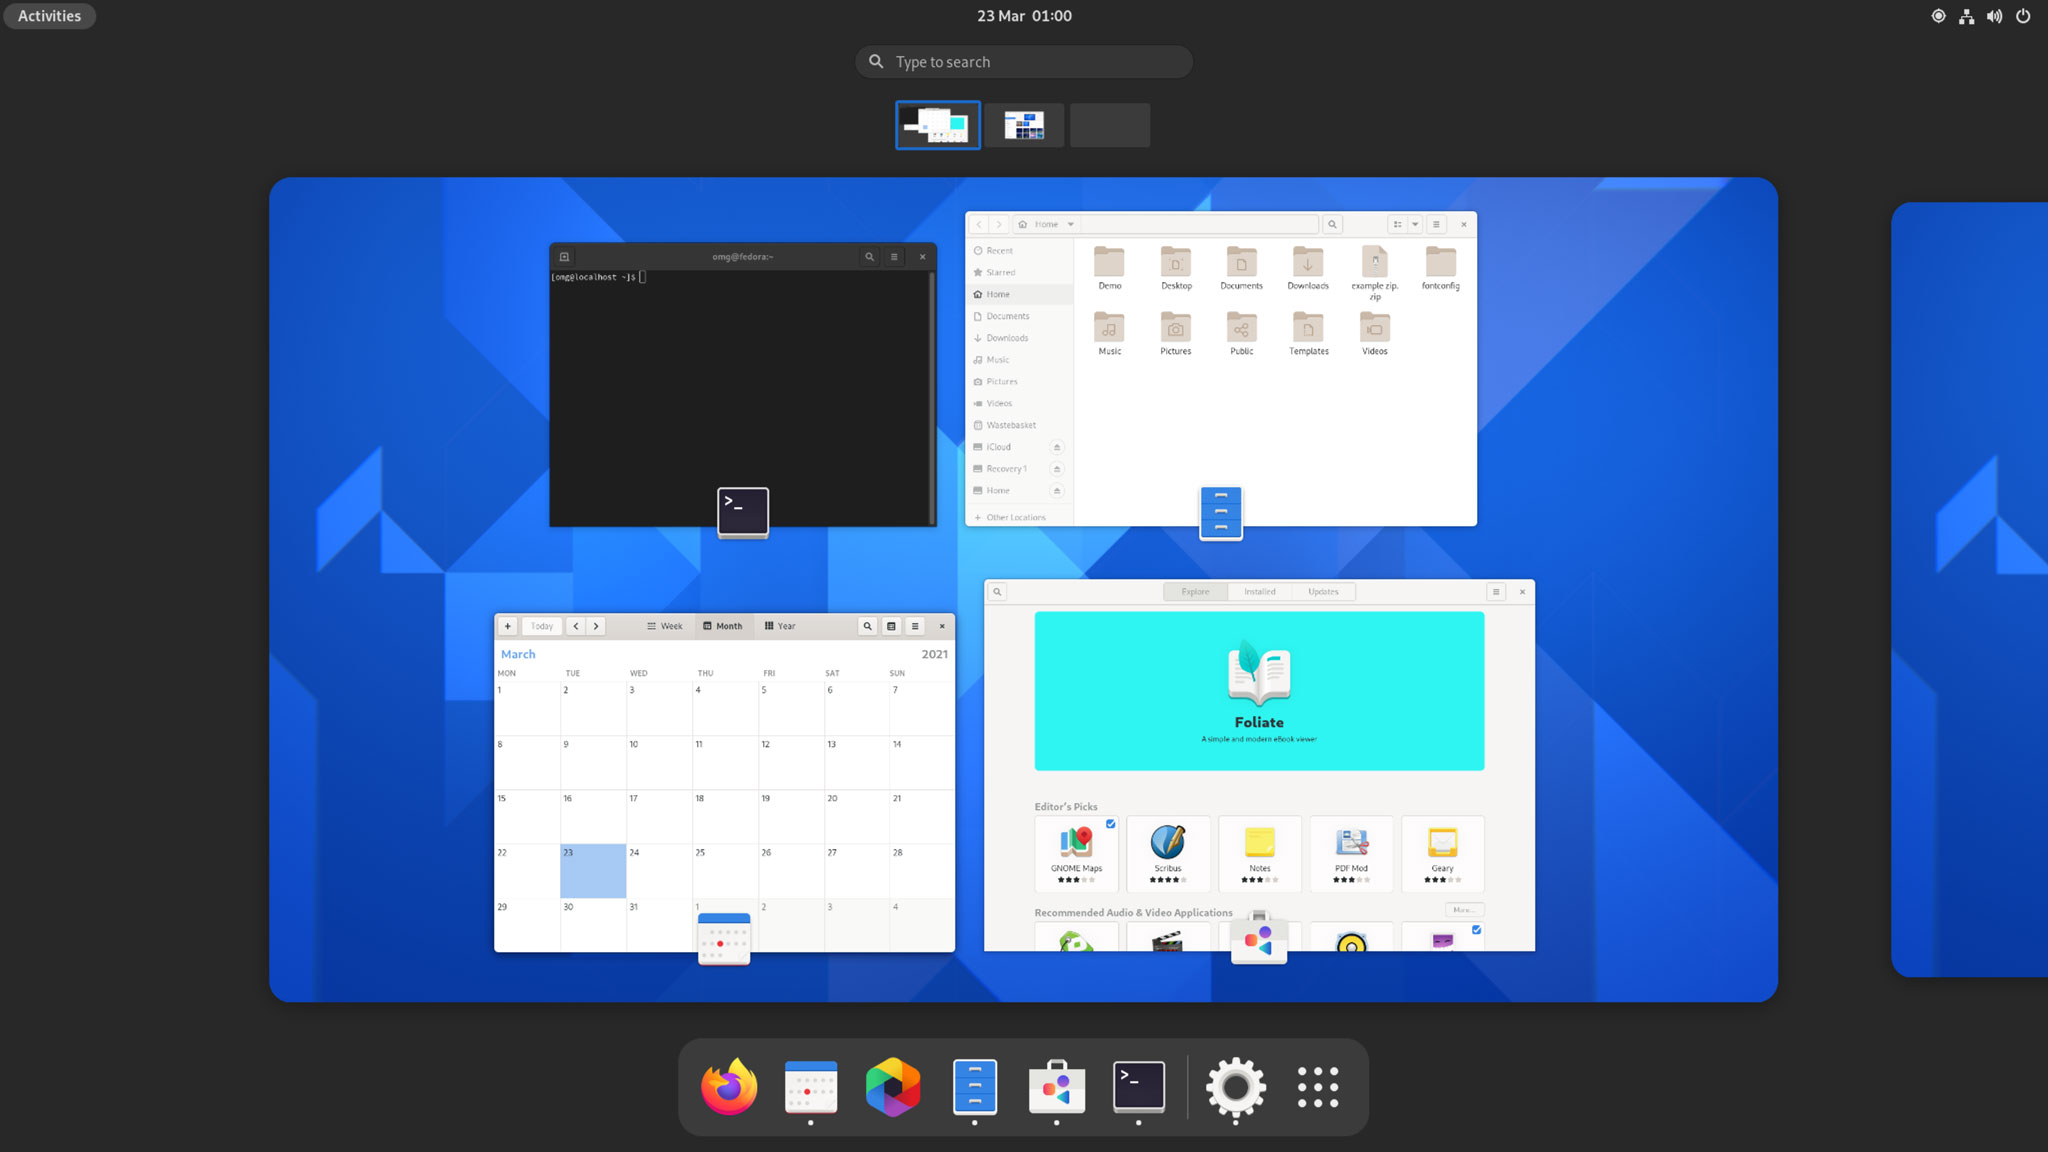
\includegraphics[width=0.9\textwidth]{img/gnome-desktop.jpg}
                \caption{\href{https://forty.gnome.org/}{Gnome 40 Desktop}}
            \end{figure}
        \end{column}
        \begin{column}{0.5\textwidth}
            \begin{figure}
                \centering
                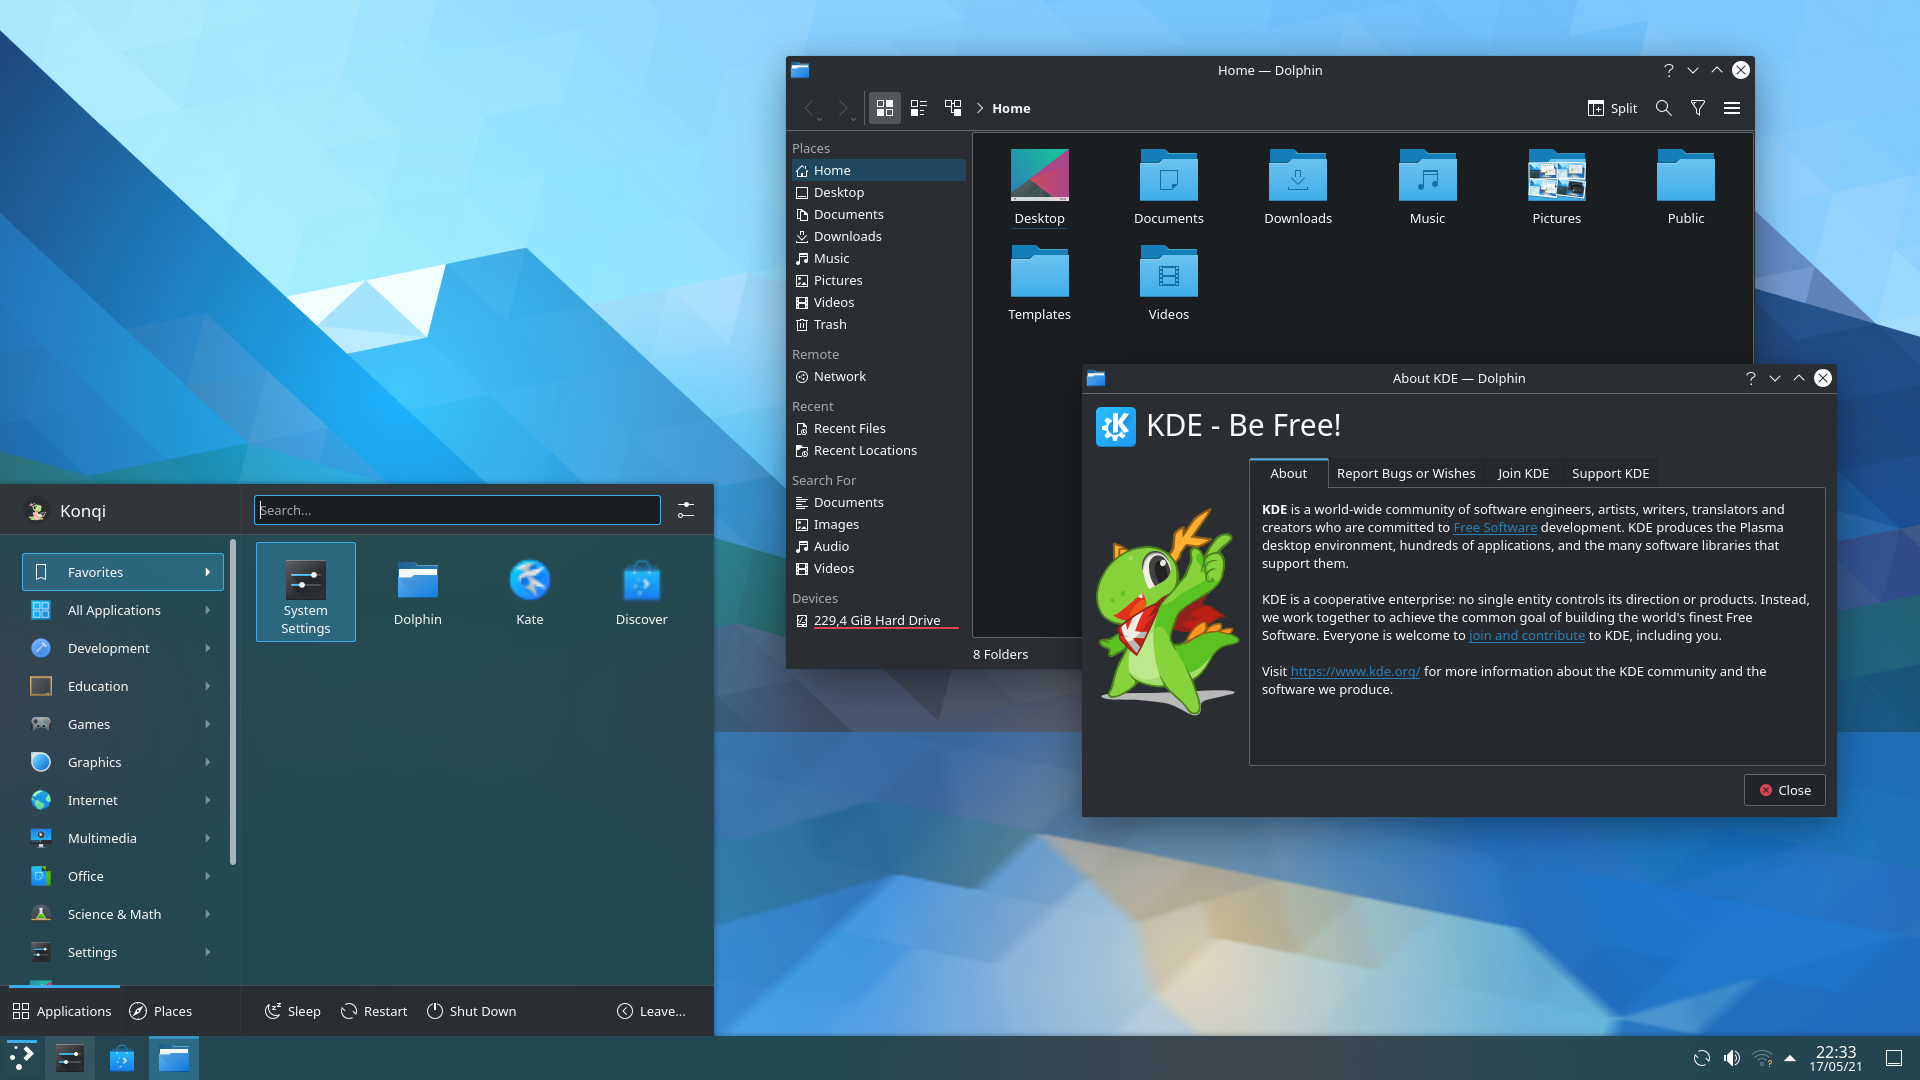
\includegraphics[width=0.9\textwidth]{img/kde_plasma.png}
                \caption{\href{https://kde.org/es/plasma-desktop/}{KDE Plasma Desktop}}
            \end{figure}
        \end{column}
    \end{columns}

\end{frame}

\begin{frame}
    \frametitle{Tiling Window Managers}
    Máximo uso del espacio de la pantalla, 100\% del tiempo (automático). Infinito control y personalización del escritorio.\\
    Todo con \textit{hotkeys} (ratón pa' qué?), pero más difícil de aprender.

    \begin{figure}
        \centering
        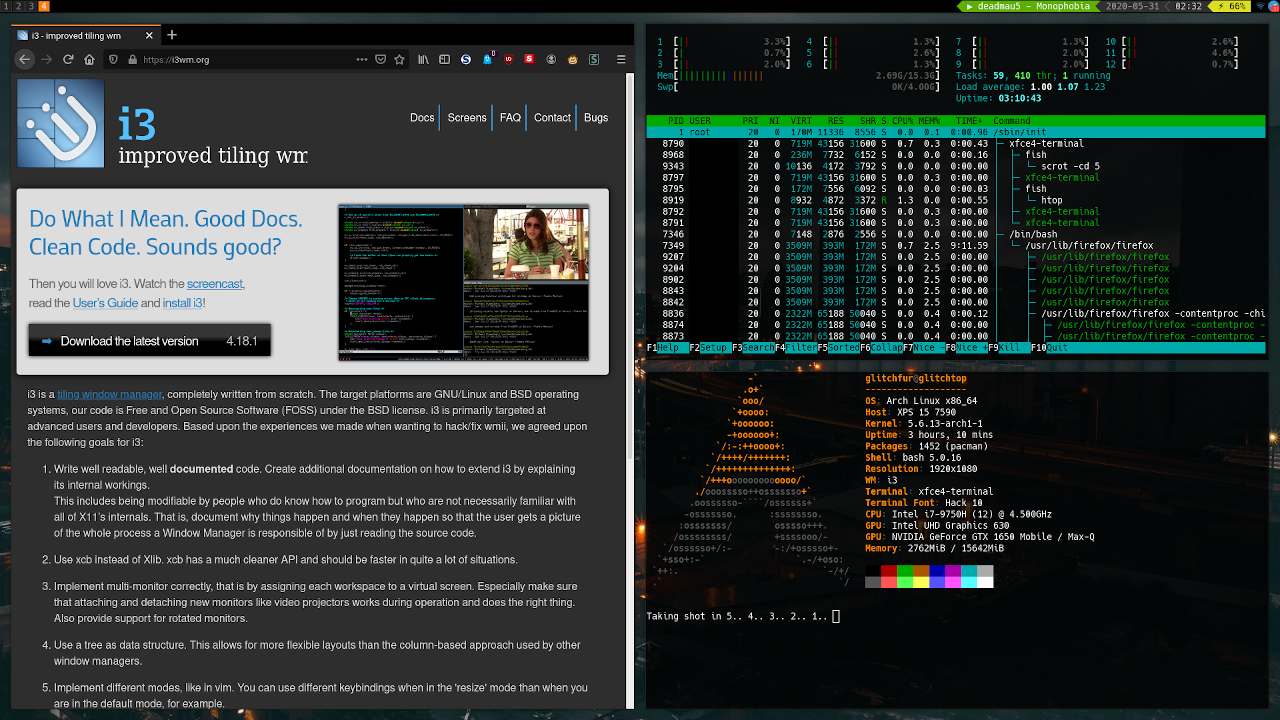
\includegraphics[width=0.6\textwidth]{img/i3_window_manager.png}
        \caption{\href{https://i3wm.org/}{i3 Window Manager}}
    \end{figure}
\end{frame}


\subsection{Emuladores de terminal}
\begin{frame}
    \frametitle{Emuladores de terminal}
    Permiten interactuar con la terminal real, y añaden muchas funcionalidades (copiar y pegar, múltiples terminales...).\newline
    
    % images
    \begin{columns}[c]
        \begin{column}{0.5\textwidth}
            \begin{figure}
                \centering
                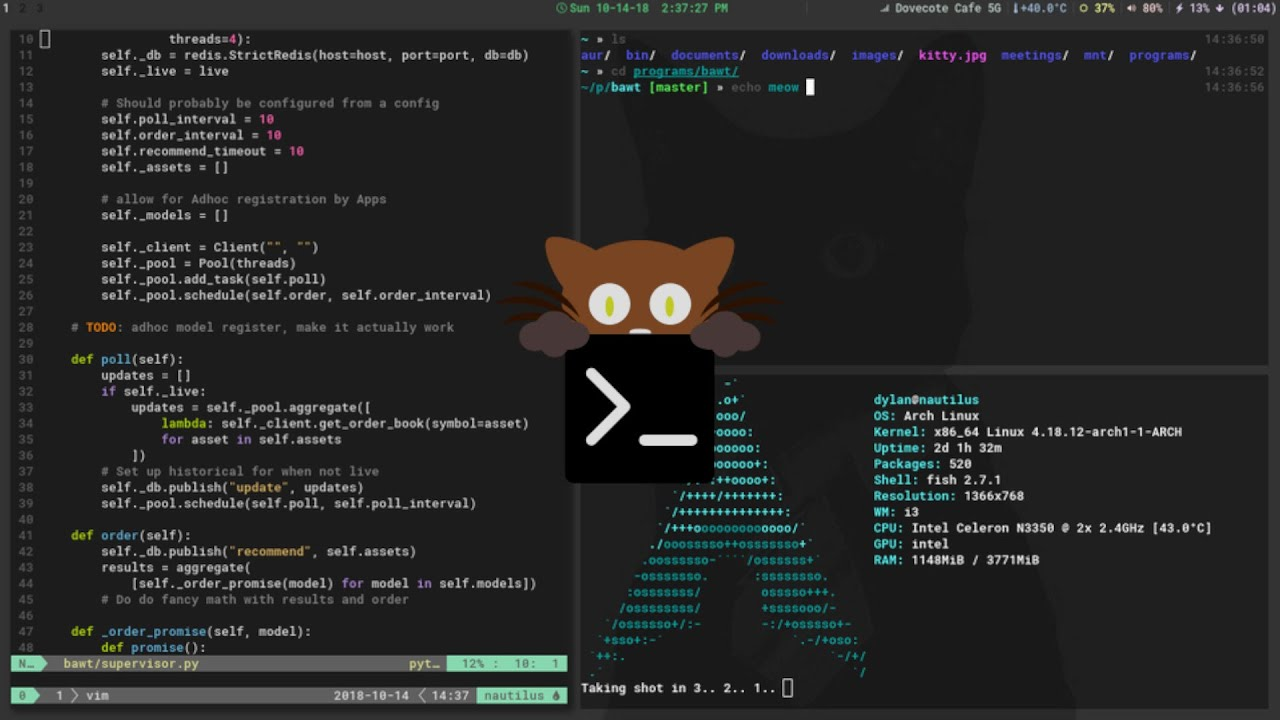
\includegraphics[width=0.9\textwidth]{img/kitty_terminal.jpg}
                \caption{\href{https://sw.kovidgoyal.net/kitty/}{Kitty}}
            \end{figure}
        \end{column}
        \begin{column}{0.5\textwidth}
            \begin{figure}
                \centering
                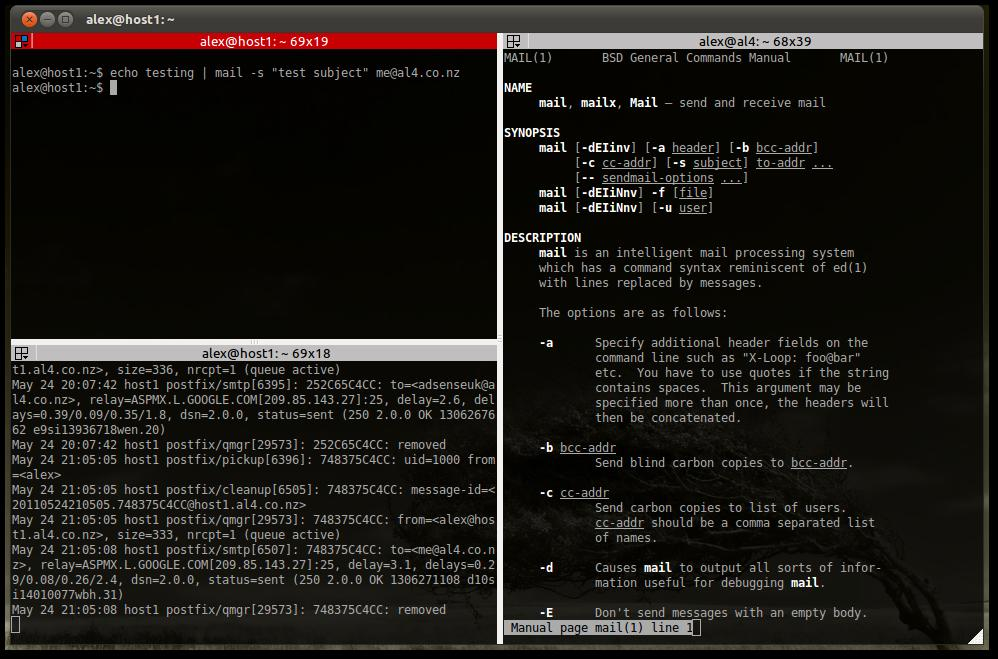
\includegraphics[width=0.9\textwidth]{img/terminator_terminal.jpg}
                \caption{\href{https://gnome-terminator.org/}{Terminator Terminal Emulator}}
            \end{figure}
        \end{column}
    \end{columns}

\end{frame}

\subsection{Shells}

\begin{frame}
    \frametitle{Shells}
    Existen distintos programas de terminal, con distintas funcionalidades (configuración, autocompletado, plugins, etc.).\\
    Son extremadamente fáciles de intercambiar (\href{https://man7.org/linux/man-pages/man1/chsh.1.html}{\texttt{chsh}}), y aún más rápido de arrancar una u otra (son programas: e.g. \href{https://www.man7.org/linux/man-pages/man1/bash.1.html}{\texttt{bash}}). 

    % images
    \begin{columns}[c]
        \begin{column}{0.5\textwidth}
            \begin{figure}
                \centering
                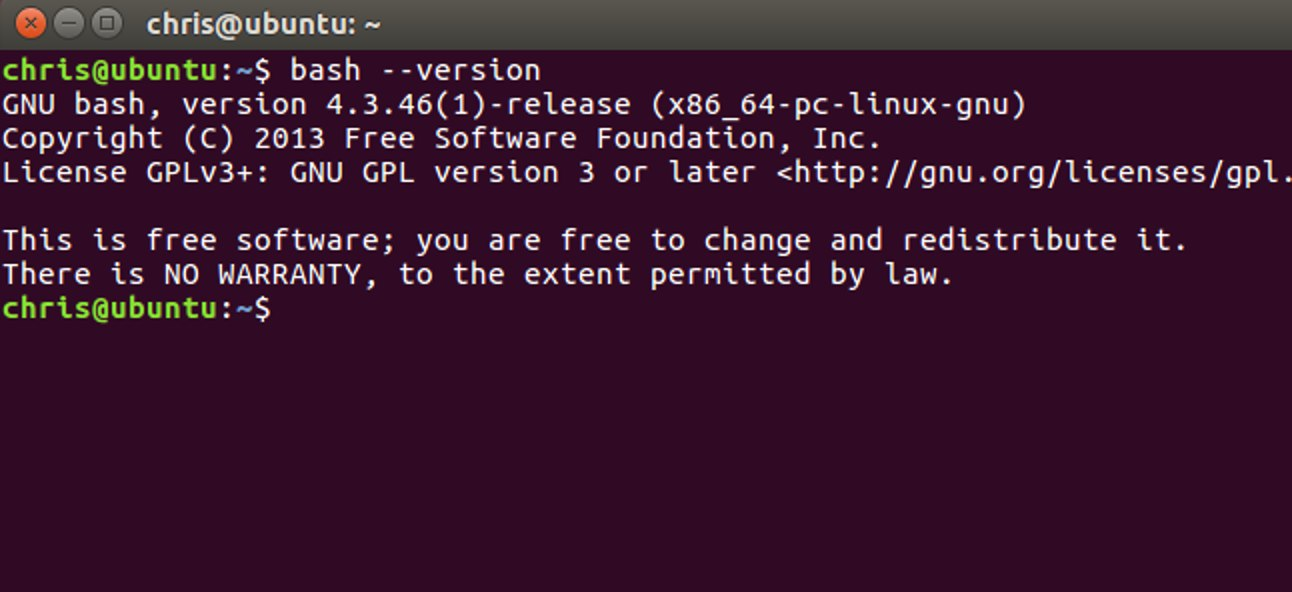
\includegraphics[width=0.9\textwidth]{img/bash_shell.jpg}
                \caption{Bash}
            \end{figure}
        \end{column}
        \begin{column}{0.5\textwidth}
            \begin{figure}
                \centering
                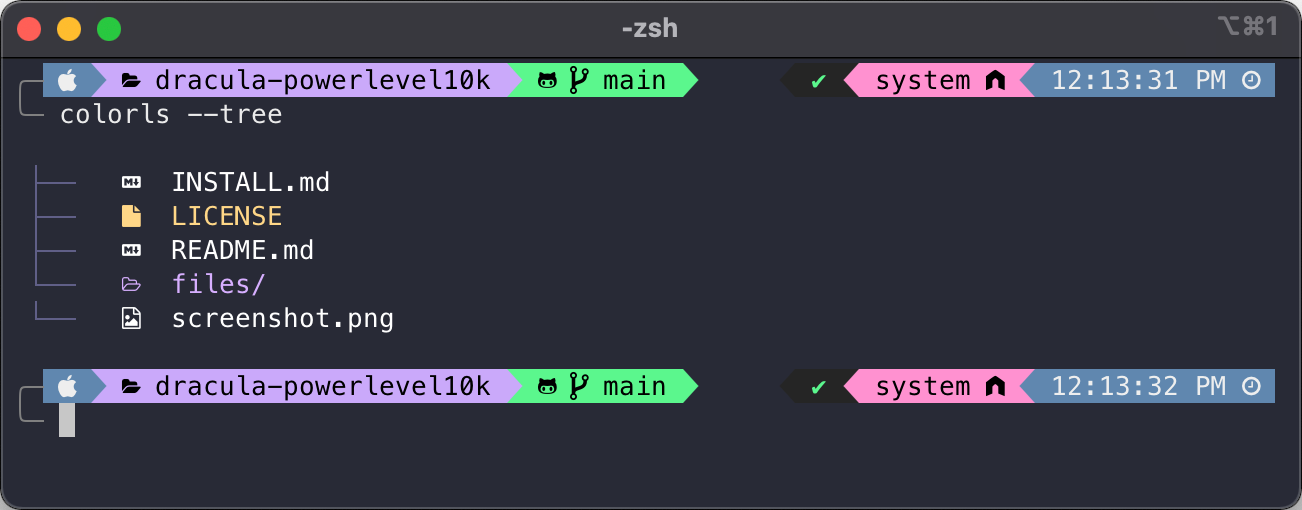
\includegraphics[width=0.9\textwidth]{img/powerlevel10k.png}
                \caption{\href{https://www.zsh.org/}{Z-Shell }\href{https://github.com/romkatv/powerlevel10k}{(with powerlevel10k)}}
            \end{figure}
        \end{column}
    \end{columns}

\end{frame}


\subsection{Dotfiles}

\begin{frame}
    \frametitle{Dotfiles}
    En Linux la mayoría de aplicaciones \textbf{guardan su configuración en archivos de texto plano}, ya sea en \texttt{/etc/} o en \texttt{/home/<user>}, y suelen llamarse "\texttt{.<program>rc}", de ahí su nombre de "\textit{resource files}" o "\textit{dotfiles}".\newline

    Ésto hace que crear, modificar, y compartir configuraciones sea muy sencillo y poderoso (\textit{scripting}, \href{https://github.com/rajayonin/dotfiles}{repositorios}, ...).

    \begin{figure}
        \centering
        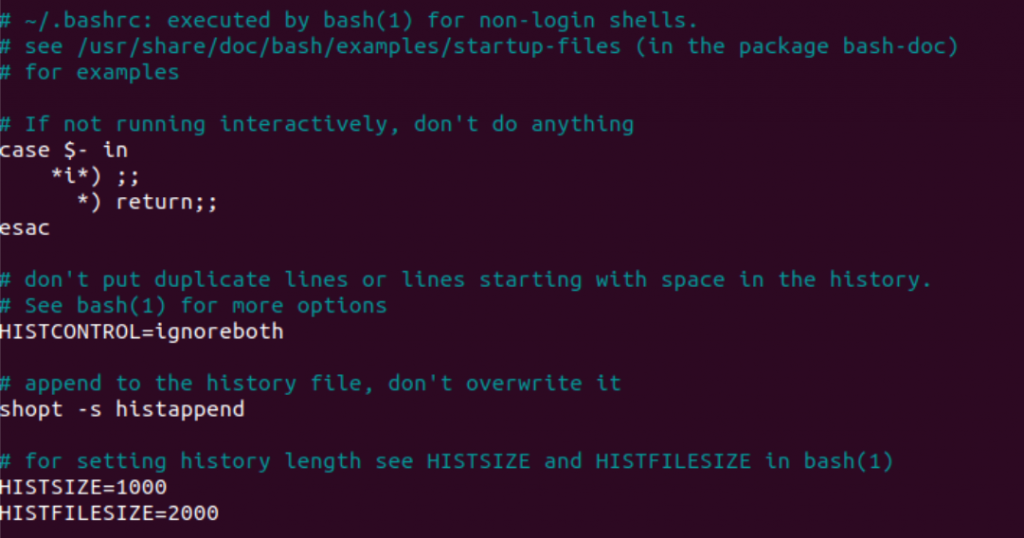
\includegraphics[width=0.4\textwidth]{img/bashrc.png}
        \caption{.bashrc}
    \end{figure}


\end{frame}


\section{La terminal}
% Sintaxis: flags, parámetros, y argumentos
% Contraseñas no se muestran en pantalla, Ctrl-L, Ctrl-C, Ctrl-D, Ctrl-Shift-C, Ctrl-Shift-V
% Funcionalidades de shell: |, >>, >, <, &&, &, nohup, Ctrl-z, fg
% Shell scripts
% Comandos (https://www.youtube.com/watch?v=s3ii48qYBxA, https://www.youtube.com/watch?v=PeCBpI1hT2Q&t=19s): 
% - Basic: ls, mv, cp, rm, cd, mkdir
% - Coreutils (https://www.maizure.org/projects/decoded-gnu-coreutils/): find/whereis, who, grep, echo, chmod, touch, cat, xxd, history, sudo, df, script
%   - Work w/ files: less, head, tail, sort, comm (diff/cmp), sed/awk, wc, cut, expand/unexpand, tee, jq, yq, xmlint
% - Processes: top (htop) / ps, lscpu,service, kill/kilall
% - Network: ping, traceroute, ipconfig, wget
% - File system: mount, fdisk/gparted, zip/unzip/tar
% - Other: lscpu, neofetch
% - Coña: cowsays, fortune, sl, cmatrix, lolcat, fortune | cowsay -f tux | lolcat (https://www.youtube.com/watch?v=iAdpkqLD4f0)
% Editores de texto en terminal: nano/micro, vim/nvim (lazyvim), emacs
% Reemplazos de comandos: exa, bat
% Configurar terminal: aliases, PS1 (prompt)

\begin{frame}
    \frametitle{La terminal}
    La principal funcionalidad de la shell/TTY/terminal es ejecutar programas.\\
    Los programas más genéricos y usados para interactuar con el SO se suelen llamar "comandos".\newline

    Por defecto busca los programas en \texttt{/usr/bin/}, pero también puedes especificar el archivo con su \textit{path} (recuerda que el archivo tiene que ser ejecutable).

\end{frame}


\begin{frame}[fragile]  % [fragile] needed for verbatim
    \frametitle{Sintaxis general}

    La sintaxis general de cualquier comando es:\\

    \begin{block}{}  % verbatim doesn't respect tabulation
        \begin{verbatim}
<command> [-<f><g>] [--<flag>] [<parameter>] [<argument>]
        \end{verbatim}
    \end{block}

    \begin{itemize}
        \item \textbf{Flags:} Son opciones del comando. Dependiendo de la opción pueden implicar la presencia de un parámetro. Pueden ser escritas con una letra (\texttt{-<f>}) o una palabra (\texttt{--<flag>}), normalmente equivalentes (e.g: \texttt{-h} y \texttt{--help}).
        \item \textbf{Parámetros:} Expanden las opciones del comando.
        \item \textbf{Argumentos:} Los \textit{inputs} del comando. Suelen ser archivos.
    \end{itemize}
    
    E.g.: \texttt{tar -rvf ../stuff.tar --exclude-from exclude\_file .}

\end{frame}


\subsection{Funcionalidades de la terminal}

\begin{frame}
    \frametitle{Funcionalidades de la terminal (I)}
    La shell también trae una serie de funcionalidades extra:

    \begin{itemize}
        \item \textbf{Concatenaciones:} Sirven para concatenar comandos:\\
        \texttt{<comm1> <cc> <comm2>}\\
        \begin{itemize}
            \item \texttt{;} ejecuta \textbf{siempre} el segundo comando cuando termina el primero.
            \item \texttt{\&\&} ejecuta el segundo comando sólo \textbf{si el primero ha funcionado} (retorna \texttt{0}).
            \item \texttt{||} ejecuta el segundo sólo \textbf{si el primero ha fallado}.
        \end{itemize}
        % E.g.: \texttt{sudo apt update \&\& apt upgrade}
        \item \textbf{Pipes:} Conectan la salida de un comando (\texttt{stdout}) a la entrada (\texttt{stdin}) del siguiente comando. Útil para enlazar comandos: \texttt{<comm1> | <comm2>}\\
        % Mítico ejemplo, buscar algo en un directorio: \texttt{ls | grep "algo"}.
        \item \textbf{Redirecciones:} Redirigen la entrada ó salida de un comando a un archivo: \texttt{<comm> <rr> <file>}.
        \begin{itemize}
            \item \texttt{>} redirige la salida de un comando a un archivo (sobreescribe).
            \item \texttt{>>} concatena la salida de un comando a un archivo (no sobreescribe).
            \item \texttt{<} redirige los contenidos de un archivo a la entrada del comando.
        \end{itemize} 
        % E.g.: \texttt{cat a >> b}

    \end{itemize}

\end{frame}

\begin{frame}
    \frametitle{Funcionalidades de la terminal (II)}

    \begin{itemize}
        \item \textbf{Sudo:} Ejecuta el siguiente comando como \textit{root}: \texttt{sudo <comm>}.
        \item \textbf{Contraseñas:} No se muestra \textit{nada} en pantalla (se puede cambiar en \texttt{/etc/sudoers} \footnote{\href{https://www.howtogeek.com/194010/how-to-make-password-asterisks-visible-in-the-terminal-window-in-linux/}{Más info aquí.}}). 
        \item \textbf{Copiar y pegar:} Se usan \texttt{Ctrl-Shift-C} y \texttt{Ctrl-Shift-V}.
        \item \textbf{Cancelar comandos:} Cancela el comando que estás ejecutando actualmente con \texttt{Ctrl-C}.
        \item \textbf{Cerrar sesión:} Cierra la sesión de terminal actual con \texttt{Ctrl-D} (útil para SSH).
        \item \textbf{Limpiar pantalla:} Limpia la pantalla con \texttt{Ctrl-L}, ó \texttt{clear}.
        \item \textbf{Borrar línea:} Borra todo el comando que estás escribiendo con \texttt{Ctrl-U}.
        \item \textbf{Autocompletado:} Con el \texttt{Tab}. Si hay más de una opción posible, tienes que darle dos veces.
    \end{itemize}

\end{frame}

\begin{frame}
    \frametitle{Funcionalidades de la terminal (III)}
    
    \begin{itemize}
        \item \textbf{Procesos en background:} 
        \item \textbf{Flechitas:} 
        \item \textbf{Repeat command:} !!, !-3
    \end{itemize}

\end{frame}


\subsection{Comandos}



\section{Permisos}
% rwx, chmod, etc.

\begin{frame}
    \frametitle{Permisos}
    
\end{frame}


\section{Más paquetes}
% Más gestores de paquetes: flatpak, snapd (malo), nix, nala (pa debian) 
% LSW ("Linux Subsystem for Windows"): wine, Lutris, heroic games, steam (proton)

\begin{frame}
    \frametitle{Más paquetes}
    
\end{frame}


\section{Configuración y ayuda}
% Ficheros de configuración: /etc/hosts
% Aiuda: man, --help, whatis

\begin{frame}
    \frametitle{Configuración y ayuda}
    
\end{frame}


\section{SSH (Secure Shell Hashing)}
% ssh, scp


\begin{frame}
    \frametitle{SSH (Secure Shell Hashing)}
    
\end{frame}



\section{Backups}
% rclone: https://www.howtogeek.com/451262/how-to-use-rclone-to-back-up-to-google-drive-on-linux/

\begin{frame}
    \frametitle{Backups: rclone}
    
\end{frame}



\begin{frame}
    \frametitle{¿Preguntas, reclamos, improperios?}
    \centering
    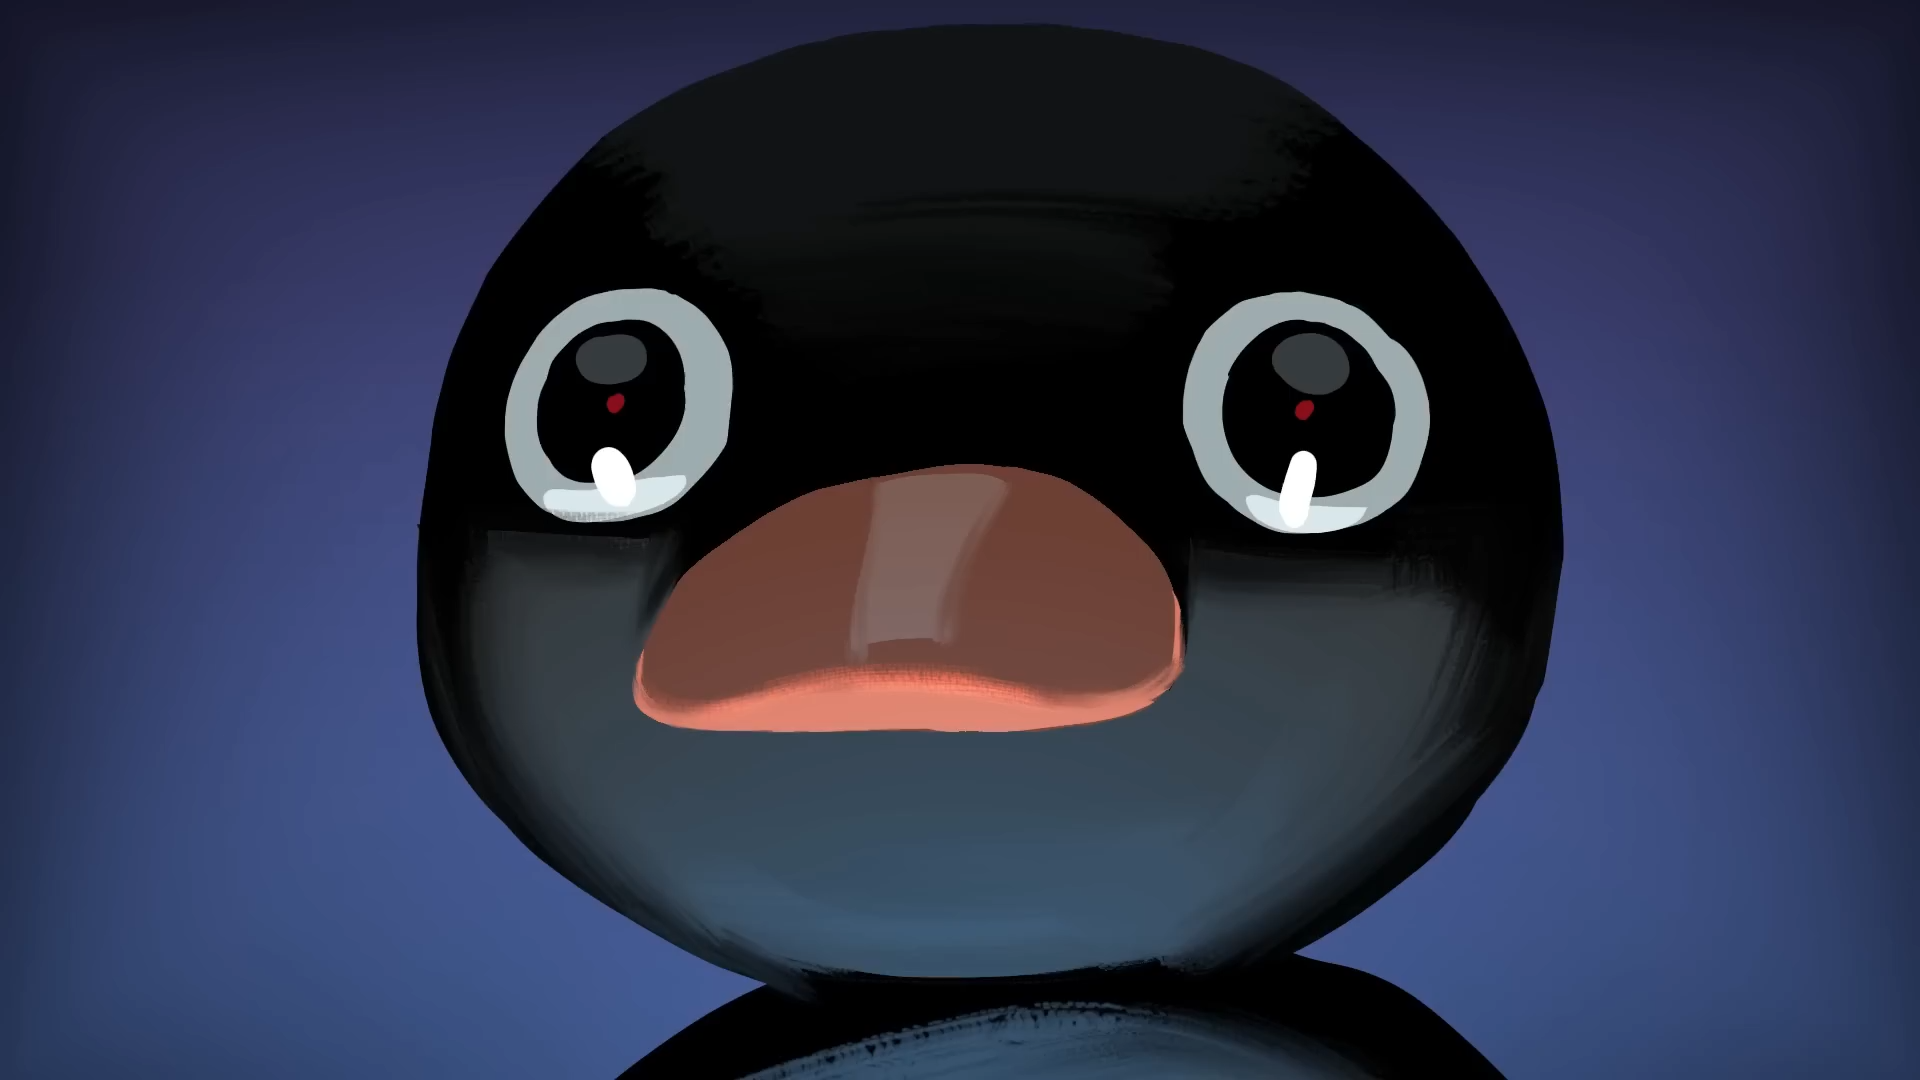
\includegraphics[width=0.9\textwidth]{img/noot.png}
\end{frame}



\begin{frame}
    \frametitle{Más información}

    \begin{itemize}
        \item \href{https://itsfoss.com/}{It's FOSS}
        \item \href{https://wiki.archlinux.org/}{Arch Wiki}
        \item \href{https://stackoverflow.com/}{Stack Overflow} y \href{https://stackoverflow.com/}{Stack Exchange}
        \item \href{https://www.tutorialspoint.com/unix/index.htm}{Tutorialspoint — Linux for Beginners}
        \item \href{https://github.com/acaldero/uc3m_linux}{A. Calderón — Introducción a Unix/Linux}
        \item \href{https://aprendolinux.com}{J. Pons — aprendolinux}
        \item \href{https://github.com/rajayonin/cheatsheets/blob/main/vim_cheatsheet.md}{L. Casais — rajayonin's Vim cheatsheet}
        \item \href{https://youtu.be/2qZBUa93MQ8}{GUL — Linux en 90' para no desesperarse en las prácticas}
        \item \href{https://cloud-gul.uc3m.es/s/4qXKozr7DmDSZiN}{GUL — Linux 404: Introducción a GNU/Linux}
        \item \href{https://github.com/guluc3m/linux404/blob/main/README.md}{GUL — Formas de instalarse Linux}
        \item \href{mailto:info@gul.uc3m.es}{info@gul.uc3m.es} | \href{https://twitter.com/guluc3m}{@guluc3m}
    \end{itemize}

\end{frame}


\begin{frame}
    \frametitle{QR}
    
\end{frame}


\end{document}
